% Numerical Computing II
% Homework 17
% Random Numbers
% February 20, 2010
% Problems 17.1,17.4,17.3 optional

\documentclass[11pt]{article}
\usepackage{listings}
\usepackage[fleqn]{amsmath}
\usepackage{graphicx}
\begin{document}         
% Start your text
\newcommand{\makehomework}[2]%
{\begin{center}%
	\Huge #1\\%
	\Large #2\\%
	Marty Fuhry\\%
	\today%
\end{center}}
\makehomework{Numerical Computing II}{Homework 17: Random Numbers}

\lstset{language=Matlab,numbers=left,frame=single,breaklines=true,morecomment=[l]{//}}
\section*{Exercise 17.1}
\lstinputlisting{problem_17_1.m}

\pagebreak
The graph produced by this code:

\begin{center}
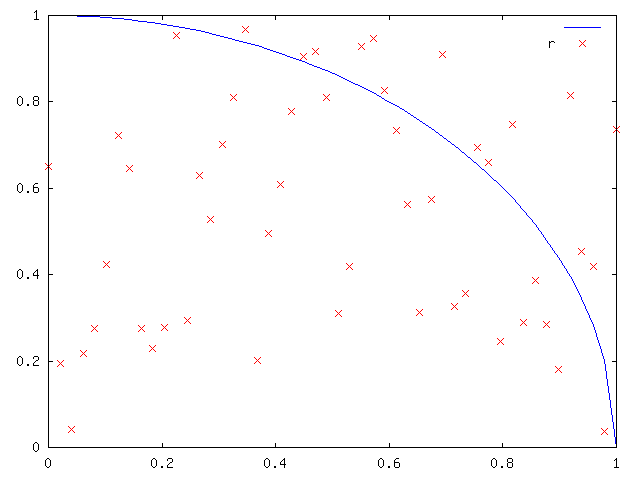
\includegraphics[scale=0.5]{problem_17_1_graph.png}
\end{center}

After running this code, we get:

\begin{align*}
	u = 36 \\
	u/n = 36/50 = 0.72000
\end{align*}

Since $\pi/4 \approx 0.78540$, our approximation of the area under the circle is very close. We
may remark that by generating more and more random values, we will
recieve closer approximations to the actual area of the quarter 
cirle. Observe what happens when we set $n = 10000$:
\begin{align*}
	u =  7885\\
	u/n = 7885/10000 = 0.78850
\end{align*}

Now, this is a very close approximation.

\pagebreak

\section*{Exercise 17.3}

	\subsection*{1. How long does it take for the sequence to repeat itself?}
	The following code generates this sequence:
	\lstinputlisting{problem_17_3.m}

	We can examine the random variables by looking at $x$:
	\begin{equation}
	x = 1, 2, 5, 6, 1, 2, 5, 6, 1, 2, 5, 6, ...
	\end{equation}

	Clearly, this repeats every 4 numbers. If we were to write out the numbers
	we would see how quickly it repeats:
	\begin{flalign*}
	&x_1 &= 1 \\
	&x_2 = (3*x_1 - 1) mod 8 = 2 mod 8 &= 2 \\
	&x_3 = (3*x_2 - 1) mod 8 = 5 mod 8 &= 5 \\
	&x_4 = (3*x_3 - 1) mod 8 = 14 mod 8 &= 6 \\
	&x_5 = (3*x_4 - 1) mod 8 = 17 mod 8 &= 1 = x_1 \\
	&x_6 = (3*x_5 - 1) mod 8 = (3*x_1 - 1) mod 8 &= 2 = x_2 \\
	\end{flalign*}

	\subsection*{2. What are the smallest and largest values in the sequence?}
	The smallest value is 1, and the largest is 6.

	\subsection*{3. Are the values in the sequence uniformly distributed in the interval
	    defined in the last question?}
	No, not in the sense of a true uniform distribution where every value is equally
	spaced from the next. However, the middle values 2 and 5 are exactly 1 away from
	the end values, so we are indeed close.

\pagebreak

\section*{Exercise 17.4}

The odds of discovering 1, 1, 0 should be the same as the odds of discovering
0, 0, 1. This is simply because we have defined which random variables should be
1 and which should be 0. Had we rounded the other way, that is, had we switched
every 1 and 0, we would duplicate our results.

Regardless, the probability of finding 1,1,0 before 0,1,1 (or vice-versa) is 
curiously low. This is not because of rarity of sequences of 1,1,0, but because
we may not allow 0,1,1 to occur before 1,1,0. That is, we may not
allow a 0 to preceed 1,1,0, or we will have formed the string 
0,1,1,0, and thus, the string 0,1,1 will be formed before 1,1,0.

The following code will stop when either a 1,1,0 or 0,1,1 sequence occurs:
\lstinputlisting{problem_17_4_either_or.m}

Running this code a few times, we rarely find either of the two sequences beyond
4 numbers into the overall sequence.

\pagebreak

We can find the number of times 0,1,1 occurs before 1,1,0 with the following code:
\lstinputlisting{problem_17_4.m}

Running this code, we find that 0,1,1 occurs before 1,1,0 a surprisingly 
high number of times. I found that 0,1,1 occurs before 1,1,0 around 
75 times in 100 tests. This is because the string 0,1,1 contains the
first two parts of the string 1,1,0. This means, in order for the 
string 1,1,0 to occur before the string 0,1,1, the string 1,1,0 needs
to be preceeded by a 1, or be the first occurance in the set. If 
1,1,0 is preceeded by a 0, then the string 0,1,1,0 is formed, and
thus 0,1,1 occurs before 1,1,0. So what we are really looking for
is either 1,1,0 occuring first or 1,1,1,0 occuring, which has much
less probability of occuring than 0,1,1. 

The same is not true for 0,1,1. We may put either a 1 or a 0 in front
of 0,1,1, and it will still occur without 1,1,0 occuring. That is,
1,0,1,1  does not stop our search; neither does 0,0,1,1.
% Stop your text
\end{document}
